\documentclass[12pt,oneside]{article}

%%%%%%%%%%%%%%%%%%%%%%%%%%%%
%%   Zur LaTeX  %%
%%%%%%%%%%%%%%%%%%%%%%%%%%%%

% Alle für die Anfertigung der Arbeit benötigten Pakete sind bereits installiert.
% Änderungen an der Vorlage sowie den Paketen sind mit dem Betreuer abzusprechen.

%%%%%%%%%%%%%%%%%%%%%%%%%%%%
%%   Zusaetzliche Pakete  %%
%%%%%%%%%%%%%%%%%%%%%%%%%%%%
\usepackage{acronym}
\usepackage{enumerate}
\usepackage{a4wide}
\usepackage{fancyhdr}
\usepackage{graphicx}
\usepackage{palatino}
\usepackage{blindtext}
\usepackage{multirow}
\usepackage[ruled, longend]{algorithm2e}
\usepackage{float}

% folgende Zeile auskommentieren für englische Arbeiten
\usepackage[ngerman]{babel}

\usepackage[T1]{fontenc}
\usepackage[utf8]{inputenc}
\usepackage[utf8]{inputenc}

%Hervorherbung für Links entfernen
%\usepackage[bookmarks]{hyperref}
\usepackage[bookmarks, pdfborder={0 0 0}]{hyperref}

\usepackage[justification=centering]{caption}
\usepackage{csquotes}

% APA Style für Bibtex
\usepackage[style=apa,natbib=true,backend=biber]{biblatex}

\DefineBibliographyStrings{german}{
  bibliography = {Literaturverzeichnis},
}
\DefineBibliographyStrings{english}{
  bibliography = {References},
}
\bibliography{literatur}

%%%%%%%%%%%%%%%%%%%%%%%%%%%%%%
%% Definition der Kopfzeile %%
%%%%%%%%%%%%%%%%%%%%%%%%%%%%%%

\pagestyle{fancy}
\fancyhf{}
\cfoot{\thepage}
\setlength{\headheight}{16pt}

%%%%%%%%%%%%%%%%%%%%%%%%%%%%%%%%%%%%%%%%%%%%%%%%%%%%%
%%  Definition des Deckblattes und der Titelseite  %%
%%  Do not edit                                    %%
%%%%%%%%%%%%%%%%%%%%%%%%%%%%%%%%%%%%%%%%%%%%%%%%%%%%%

\newcommand{\UDOTitle}[9]{

  \thispagestyle{empty}
  
\includegraphics[width=3in]{abbildungen/tud_logo_rgb.jpg}
  \vspace*{\stretch{1}}
  \\
  {\parindent0cm
  \rule{\linewidth}{.1ex}}
  \begin{flushright}
    \vspace*{\stretch{1}}
    \sffamily\bfseries\Huge
    #1\\
    \vspace*{\stretch{1}}
    \sffamily\bfseries\large
    #2\\
    \vspace*{\stretch{1}}
  \end{flushright}
  \rule{\linewidth}{.1ex}

  \vspace*{\stretch{1}}
  \begin{center}

    \vspace*{\stretch{1}}
    \large #5\\

    \vspace*{\stretch{1}}
    \large Studiengang: #4 \\[1mm]
    \large Matrikelnummer: #3\\[1mm]
    \large Erstgutachter:  #8 \\[1mm]
    \large Zweitgutachter:  #9 \\[1mm]

    \vspace*{\stretch{1}}
    \large Bearbeitungszeit: #6 -- #7

    \vspace*{\stretch{2}}
    \large Lehrstuhl 11\\
    \large Fakultät für Informatik\\
  \end{center}
}


%%%%%%%%%%%%%%%%%%%%%%%%%%%%
%%  Beginn des Dokuments  %%
%%%%%%%%%%%%%%%%%%%%%%%%%%%%

\begin{document}
\sloppy

  \UDOTitle
      {Parallelisierung einer speichereffizienten Approximation der LZ77-Faktorisierung}                            % Titel der Arbeit
      {Sivarajah, Gajann}                           % Vor- und Nachname des Autors
      {168246}                                     % Matrikelnummer des Autors
      {Bachelor Angewandte Informatik}     % Studiengang
      {Bachelorarbeit}   % Art der Arbeit
      {30.04.2024}                                  % Tag der Anmeldung
      {30.08.2024}                                  % Tag der Abgabe
      {Prof. Dr. Johannes Fischer}                % Name des Erstgutachters
      {M.Sc. Patrick Dinklage}                                        % Name des Zweitgutachters
      
  \clearpage

\lhead{}
\pagenumbering{Roman} 
    \setcounter{page}{1}

\tableofcontents
\clearpage

\addcontentsline{toc}{section}{\listfigurename}
\listoffigures
\clearpage

\addcontentsline{toc}{section}{\listtablename}
\listoftables
\clearpage

\addcontentsline{toc}{section}{Abkürzungsverzeichnis}
% !TEX root = main.tex

\section*{Abkürzungsverzeichnis}
% nur bei Bachelor- und Masterthesis notwendig. Kommentieren sie diesen Bereich aus oder löschen Sie den INHALT dieser Datei, wenn sie eine andere Leistung (beispielsweise Seminararbeit) erbringen.

\begin{acronym}[BPM] %Wert in eckiger Klammer ist durch die längste Abkürzung zu substituieren (Anzahl der Ziffern = Breite der linken Tabellenspalte)

\acro{AI}{Artificial Intelligence}
\acro{BPM}{Business Process Management}
\acro{DSR}{Design Science Research}

\end{acronym}
\clearpage

% Formelverzeichnis können an dieser Stelle sinnvolle Ergänzungen sein.

%%%%%%%%%%%%%%%%%%%%%%%%%%%%
%%  Zusammenfassung   %%
%%%%%%%%%%%%%%%%%%%%%%%%%%%%
\markboth{Zusammenfassung}{Zusammenfassung}
\section*{Zusammenfassung}

Die Zusammenfassung dient dem Leser dazu, einen groben Überblick über die Inhalte zu gewinnen (kurze Problemstellung, Herangehensweise, Lösungsansätze und evtl. der Schlüsselerkenntnisse). Der Umfang sollte ca. eine halbe Seite betragen. Auf der nächsten Seite soll eine Übersetzung der Zusammenfassung als Abstract in englischer Sprache erfolgen.

Allgemeiner Hinweis: Die ``neue'' Rechtschreibung bietet viele alternative Möglichkeiten der Rechtschreib. Es ist demnach egal, ob Sie z.B. Potenzial mit ``z'' oder Potential mit ``t'' schreiben. Auch das Komma kann vor einem erweiterten Infinitiv wahlweise gesetzt oder weggelassen werden. Alternative Schreibweisen bedeuten zugleich aber nicht Beliebigkeit. Sie sollten sich also immer konsequent während der gesamten Arbeit für eine Schreibweise entscheiden. Dieses gilt auch für Fachbegriffe.

\clearpage

%%%%%%%%%%%%%%%%%%%%%%%%%%%%
%%  Abstract   %%
%%%%%%%%%%%%%%%%%%%%%%%%%%%%
\markboth{Abstract}{Abstract}
\section*{Abstract (nur bei Bachelor- und Masterthesis)}
Zusammenfassung in englischer Sprache.

%%%%%%%%%%%%%%%%%%%%%%%%%%%%
%%  Einstellungen  %%
%%%%%%%%%%%%%%%%%%%%%%%%%%%%
\cleardoublepage
\pagenumbering{arabic}  
    \setcounter{page}{1}
\lhead{\nouppercase{\leftmark}}

%%%%%%%%%%%%%%%%%%%%%%%%%%%%
%%  Segmentierung  %%
%%%%%%%%%%%%%%%%%%%%%%%%%%%%

%Kapitel mit Seitenumbruch
% einleitung.tex
\chapter{Einleitung}
\section{Motivation und Hintergrund}
Die Entwicklung, Verbreitung und Nutzung digitaler Technologien hängt im hohen Maße von der Fähigkeit ab, große Mengen an Daten speichern, transportieren und
analysieren zu können. Der Umgang mit großen Datenmengen geht jedoch mit entsprechend hohen Kosten einher. Ein wichtiges Werkzeug zur Bewältigung dieses Problems
sind Kompressionstechniken, die Relationen und Redundanzen in Datenmengen extrahieren, um ihre Größe möglichst auf ihre inhärente Komplexität zu reduzieren. 
Im Laufe der Zeit wurden zahlreiche Kompressionsalgorithmen entwickelt, die wiederum über mehrere Iterationen verbessert wurden.Viele solcher Kompressionstechniken
können der Familie der LZ77-Algorithmen \cite{LemZiv} zugeordnet werden, wobei diese sich in Statistiken, wie der Laufzeit, der Speicheranforderung oder Kompressionrate unterscheiden
. In \cite{ApproxLZ77} wird eine Variante der LZ77-Faktorisierung beschrieben, die über drei Phasen eine 2-Approximation einer exakten LZ77-Faktorisierung
 \cite{exactLemZiv} erreichen kann. Diese beschränkten Einbußen in der Qualität der Ausgabe werden jedoch dadurch kompensiert, dass der Algorithmus die Speicheranforderung
weit unterbieten kann. In dieser Arbeit untersuchen wir diesen Algorithmus auf ihr Potential zur Parallelisierung.

\section{Ziele und Methodik}
Im Rahmen der Parallelisierung des approximativen LZ77-Algorithmus werden wir die erste Phase des Algorithmus dahingehend anpassen, dass mehrere Threads im 
shared-memory-Modell konfliktfrei auf Datenstrukturen zugreifen und eine korrekte Ausgabe liefern können. Im Rahmen der praktischen Evaluation der
beschriebenen Konzepte wird eine Implementierung in C++ herangezogen. Die Parallelisierung wird hauptsächlich über OpenMP-Instruktionen \cite{openmp} realisiert.
Im Rahmen dieser Arbeit wird insbesondere die parallele Generierung einer Suchtabelle von Referenzen, sowie die parallele Suche nach Referenzen über die gesamte Eingabe
hinweg betrachtet. Wir führen eine theoretische und praktische Evaluation der Qualität und Performanz der Algorithmen durch. Insbesondere stellen wir einen Vergleich der
Laufzeit und Speicheranforderung der sequentiellen und parallelen Approximation mit einer exakten LZ77-Faktorisierung \cite{exactLemZiv} an. Die Güte der Parallelisierung
werden wir anhand der gemessenen Beschleunigung der Laufzeit bewerten. Für jegliche Messungen verwenden wir Testdaten aus unterschiedlichen Kontexten des 
Pizza\& Chili Corpus \cite{corpus}.
\section{Grundlagen} \label{grundlagen}

Direkt unterhalb der Hauptkapitel ist jeweils Platz für eine kurze inhaltliche Überleitung.

\subsection{Unterabschnitt}

Die Überschriftenstrukturierung ist hierarchisch. Es empfiehlt sich, die Arbeit so zu strukturieren, dass der Text immer auf der untersten Ebene steht und zugleich auf gleichen Hierarchieebenen inhaltlich auf gleicher Ebene verfasste Texte stehen. Kapitelüberschriften sind so zu wählen, dass sie sinnvoll den Inhalt des (Unter)Kapitels als Aussage wiedergeben. Die Kapitelüberschriften sind in den Formatvorlagen namentlich als Überschrift 1, Überschrift 2, usw. hinterlegt.

Eine Untergliederung bis zur dritten Ebene ist für Bachelor- und Masterarbeiten sinnvoll. Es empfiehlt sich, eine vierte Ebene (z.B. 2.1.1.1) zu vermeiden, um die Übersichtlichkeit der Gliederung zu wahren.

Ihr Text sollte unter Einbindung von Grafiken und Tabellen in Absätze gegliedert werden. Dabei ist zu beachten, dass ein Absatz einen thematischen Gedanken erfasst, wobei am Anfang des Absatzes im Regelfall die Kernaussage zu finden ist und von dieser ausgehend durch weitere Erörterungen innerhalb des Absatzes gegliedert wird.

\subsection{Unterabschnitt zwei}

\subsubsection{UnterUnterabschnitt}

\textbf{So wird dick geschrieben} und \textit{so kursiv}. \citet[685]{janiesch2021machine} so wird Autor, Jahr und Seite zitiert. So wird in Klammern zitiert: \citep[685]{janiesch2021machine} bei einer Quelle oder (\cites[685]{janiesch2021machine}[289]{herm2021symbolic}) bei mehreren. So wird eine Internetquelle zitiert: \citet{diewi}. So wird im Dokument referenziert: Kapitel \ref{einleitung}, Gleichung \ref{eq:1} zeigt...
So nutzen Sie Abkürzungen: \ac{AI}, \ac{BPM}, \ac{DSR} Achten Sie darauf, die Abkürzung in der acronym.tex zu definieren. Im Fließtext verwendete und nicht definierte Abkürzungen (und vice veresa) werden andernfalls nicht gelistet und verursachen eine Fehlermeldung. Tip: Abkürzung bei \textbf{jeder Verwendung} mit \begin{verbatim} 
    \ac{abkürzung}
\end{verbatim} definieren. Abkürzung wird dann beim ersten Auftreten automatisch eingeführt und ansonsten als Akronym kompiliert.

\newpage
So schreiben und nummerieren sie eine Formel.

\begin{equation}
    \sum_{i=1}^N x_i
    \label{eq:1}
\end{equation}
\newline//

So legen sie eine \textbf{nummerierte} Auflistung an. Substituieren Sie \textit{enumerate} mit \textit{itemize}, um Bulletpoints (\textbullet) zu verwenden.

\begin{enumerate}
\item Element 1
\item Element 2
\end{enumerate}

So fügen sie eine Abbildung ein. Achten sie darauf, dass die Breite der Abbildung \textbf{nicht} die Textbreite übersteigt (width zwischen 0.0 und 1.0). Die Abbildung wird automatisch zentriert.

\begin{figure}[H]
    \centering
    
\includegraphics[width=0.3\textwidth]{abbildungen/tud_logo_rgb.jpg}
    \caption[Kurze Caption für Inhaltsverzeichnis]{Lange Caption unter der Abbildung mit Quelle}
    \label{fig:my_label}
\end{figure}

Wichtig ist, Abbildungen immer im Text zu erläutern und im Text auf die Abbildung zu verweisen (siehe Abbildung \ref{fig:my_label}). Dies gilt auch für Tabellen. Bei fremden Abbildungen und Tabellen ist zudem die ursprüngliche Quelle anzugeben (z.B. in Klammern am Ende der Bezeichnung).

So schreibt man einen Algorithmus.
\BlankLine
\begin{algorithm}[H]
 \KwData{this text}
 \KwResult{how to write algorithm }
 initialization\;
 \While{not at end of this document}{
  read current\;
  \eIf{understand}{
   go to next section\;
   current section becomes this one\;
   }{
   go back to the beginning of current section\;
  }
 }
 \caption{How to write algorithms}
\end{algorithm}
\BlankLine
\BlankLine
So gestaltet man eine Tabelle. Achten sie darauf, dass die Breite der Tabelle die Textbreite übersteigt. Die Tabelle wird automatisch zentriert.
\begin{table}[H]
\caption[Kurze Caption für Inhaltsverzeichnis]{Lange Caption über der Tabelle, ggf. mit Quelle}
\centering
\begin{tabular}{llr}
\hline
Animal    & Description & Price (\$) \\
\hline
Gnat      & per gram    & 13.65      \\
          & each        & 0.01       \\
Gnu       & stuffed     & 92.50      \\
Emu       & stuffed     & 33.33      \\
Armadillo & frozen      & 8.99       \\
\hline
\end{tabular}
\end{table}

\subsubsection{UnterUnterabschnitt zwei}

Ein Abschnitt steht nie allein.
\section{Fazit} \label{Fazit}

In das Fazit sollen
\begin{itemize}
\item die Themenstellung
\item der gewählte Ansatz
\item die Ergebnisse der Arbeit
\item eine kritische Stellungnahme/Einschätzung sowie die Limitationen Ihrer Forschung
\item nächste Schritte
\end{itemize}
deutlich werden.
Es ist keine Nacherzählung dessen, was sie chronologisch aufgeschrieben haben.

\textbf{Hinweis:}
Die Schlussfolgerung sollte mit der Zusammenfassung bzw. dem Abstract und der Einleitung abgeglichen werden. Es sollte immer eine Zusammenfassung der wesentlichen Erkenntnisse der eigenen Arbeit sein, die den Forschungsbeitrag darstellt. Der Umfang der Schlussfolgerung sollte ähnlich wie die Einleitung ca. 5\% der gesamten Arbeit betragen.


Bitte Rechtschreibprüfung nicht vergessen.

%%%%%%%%%%%%%%%%%%%%%%%%%%%%
%% Literaturverzeichnis wird 
%% automatisch eingefügt
%%%%%%%%%%%%%%%%%%%%%%%%%%%%
\clearpage
\lhead{}
\addcontentsline{toc}{section}{\bibname}
\printbibliography

\newpage
\addcontentsline{toc}{section}{Anhang}
% anhang.tex
\chapter{Weitere Informationen}
\section{Alternative Eingabedaten} \label{alternative}
Im Folgenden sind die vollständigen Laufzeitmessungen für die Eingabedaten, sources, english, dna und xml, aufgeführt. Während die absoluten Werte
der Laufzeit für die verschiedenen Eingabedaten variieren, zeigen die Kurven der Laufzeitmessungen eine ähnliche Tendenz.
\begin{figure} [H]
    \centering
    \caption{Laufzeitmessung von LZ77, Approx.LZ77 und Approx.LZ77Par(16 Threads) auf verschiedenen Präfixen von sources. Als Vergleichsmaß wurde 
    die lineare Regression der Kurven gestrichelt eingezeichnet.}
    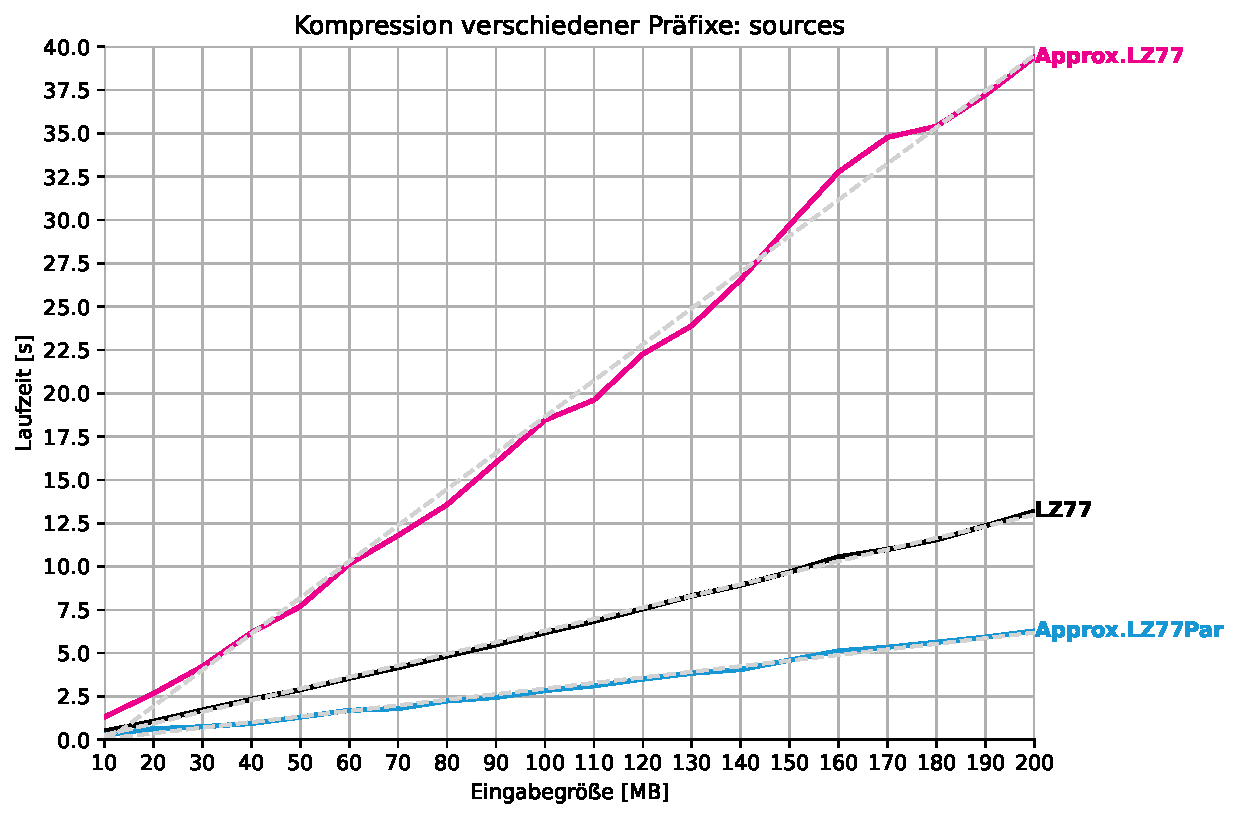
\includegraphics[scale=0.65]{Images/progressive_sources.pdf}
\end{figure}

\begin{figure}[H]
    \centering
    \caption{Laufzeitmessung von Approx.LZ77Par mit verschiedener Anzahl an Threads für sources}
    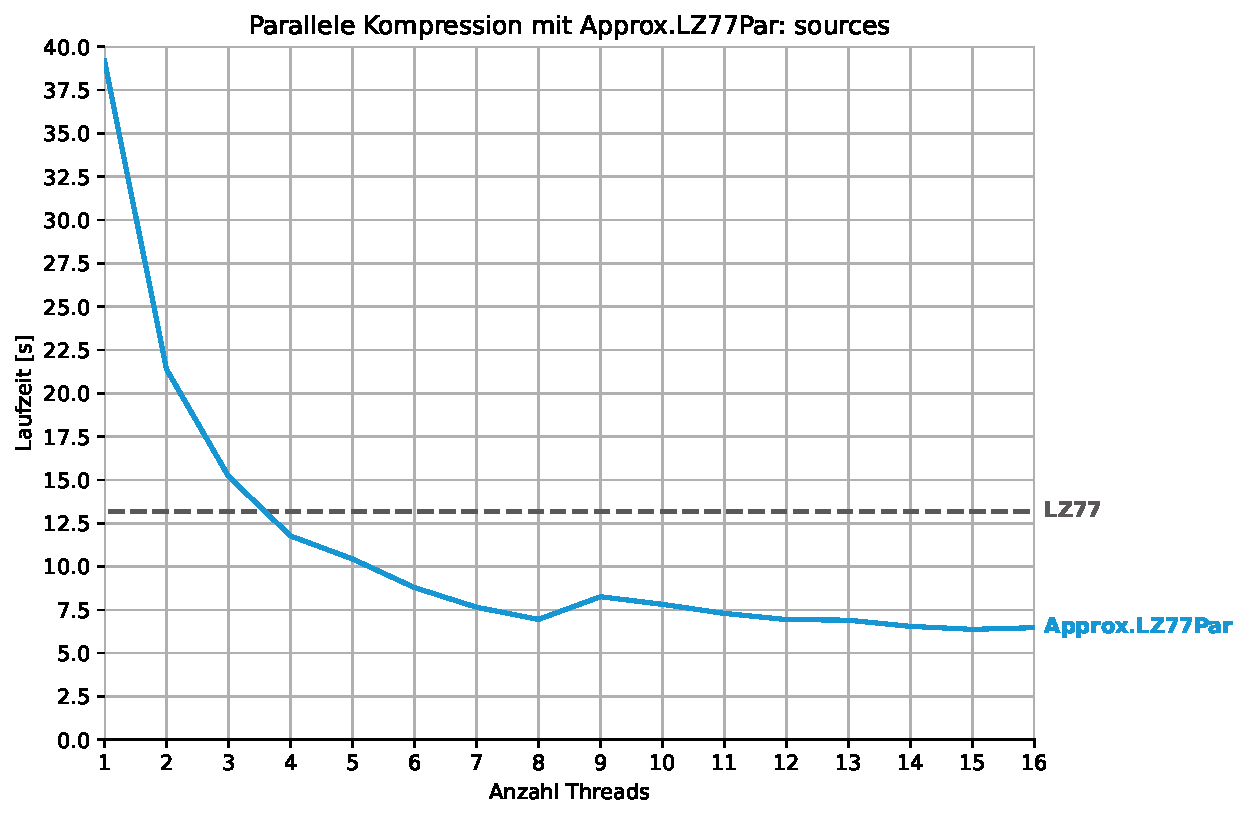
\includegraphics[scale=0.65]{Images/progressive_speedup_sources.pdf}
\end{figure}

\begin{figure}[H]
    \centering
    \caption{Laufzeitmessung von LZ77, Approx.LZ77 und Approx.LZ77Par(16 Threads) auf verschiedenen Präfixen von english. Als Vergleichsmaß wurde 
    die lineare Regression der Kurven gestrichelt eingezeichnet.}
    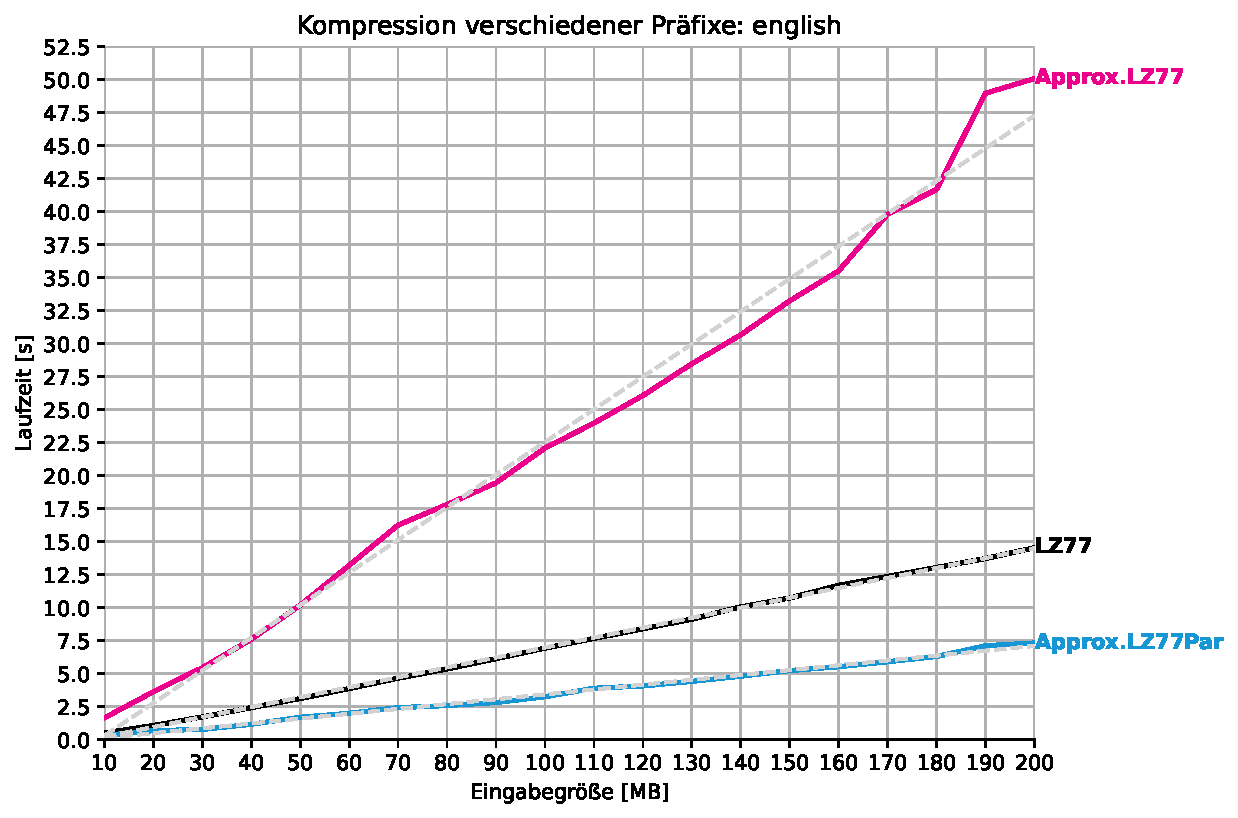
\includegraphics[scale=0.65]{Images/progressive_english.pdf}
\end{figure}

\begin{figure}[H]
    \centering
    \caption{Laufzeitmessung von Approx.LZ77Par mit verschiedener Anzahl an Threads für english}
    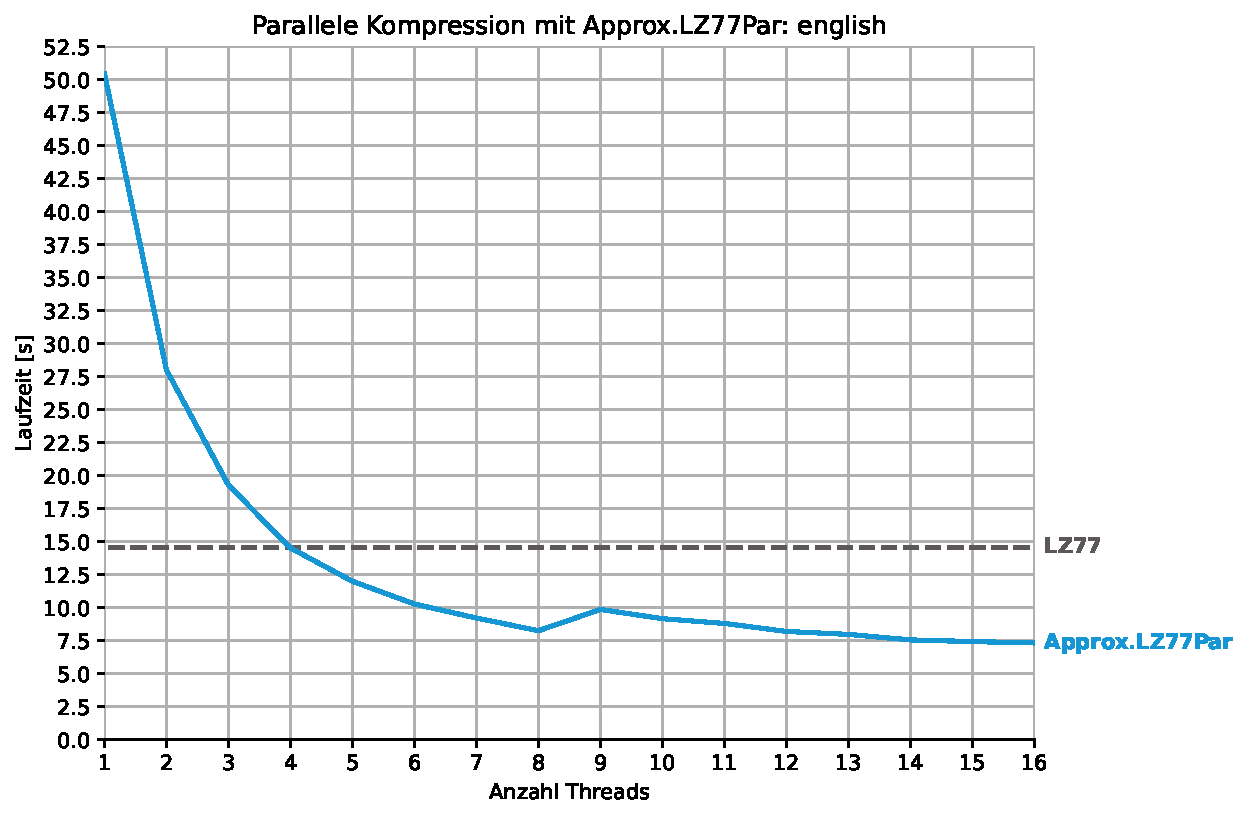
\includegraphics[scale=0.65]{Images/progressive_speedup_english.pdf}
\end{figure}

\begin{figure}[H]
    \centering
    \caption{Laufzeitmessung von LZ77, Approx.LZ77 und Approx.LZ77Par(16 Threads) auf verschiedenen Präfixen von dna. Als Vergleichsmaß wurde 
    die lineare Regression der Kurven gestrichelt eingezeichnet.}
    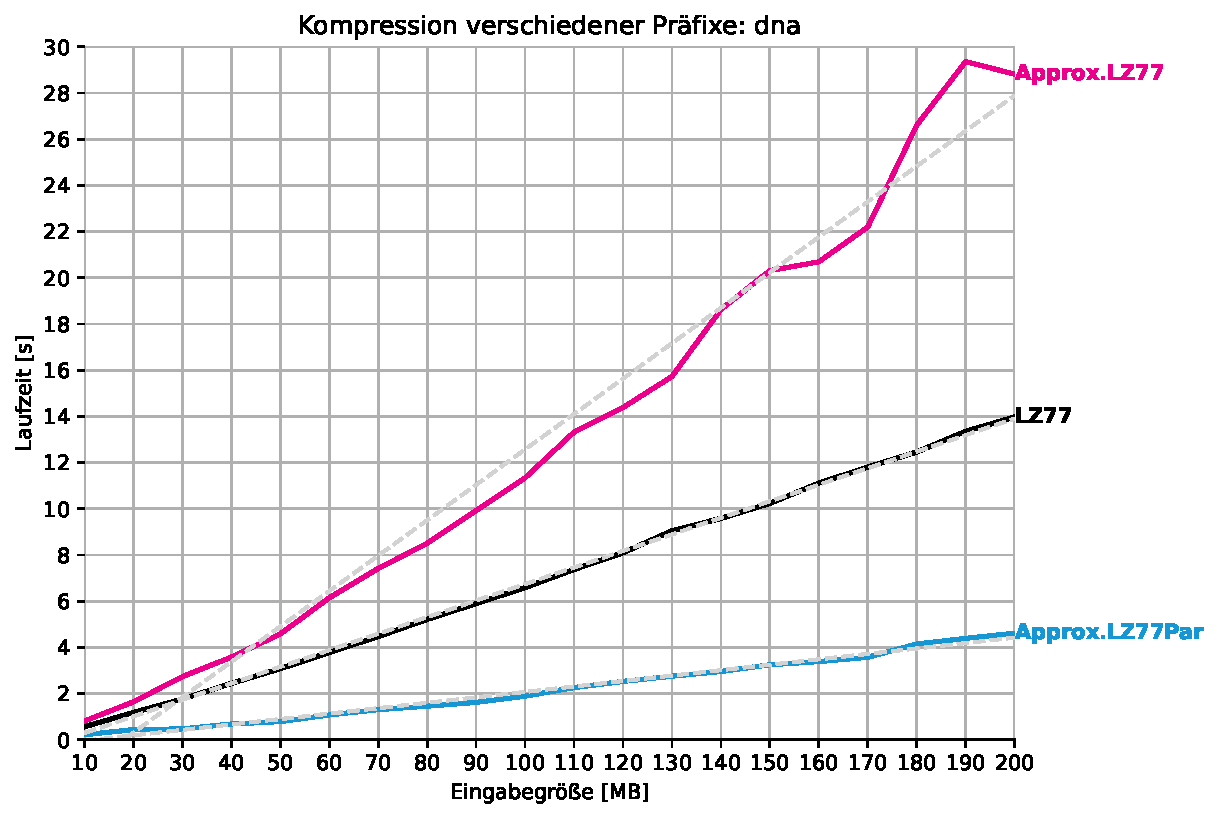
\includegraphics[scale=0.65]{Images/progressive_dna.pdf}
\end{figure}

\begin{figure}[H]
    \centering
    \caption{Laufzeitmessung von Approx.LZ77Par mit verschiedener Anzahl an Threads für dna}
    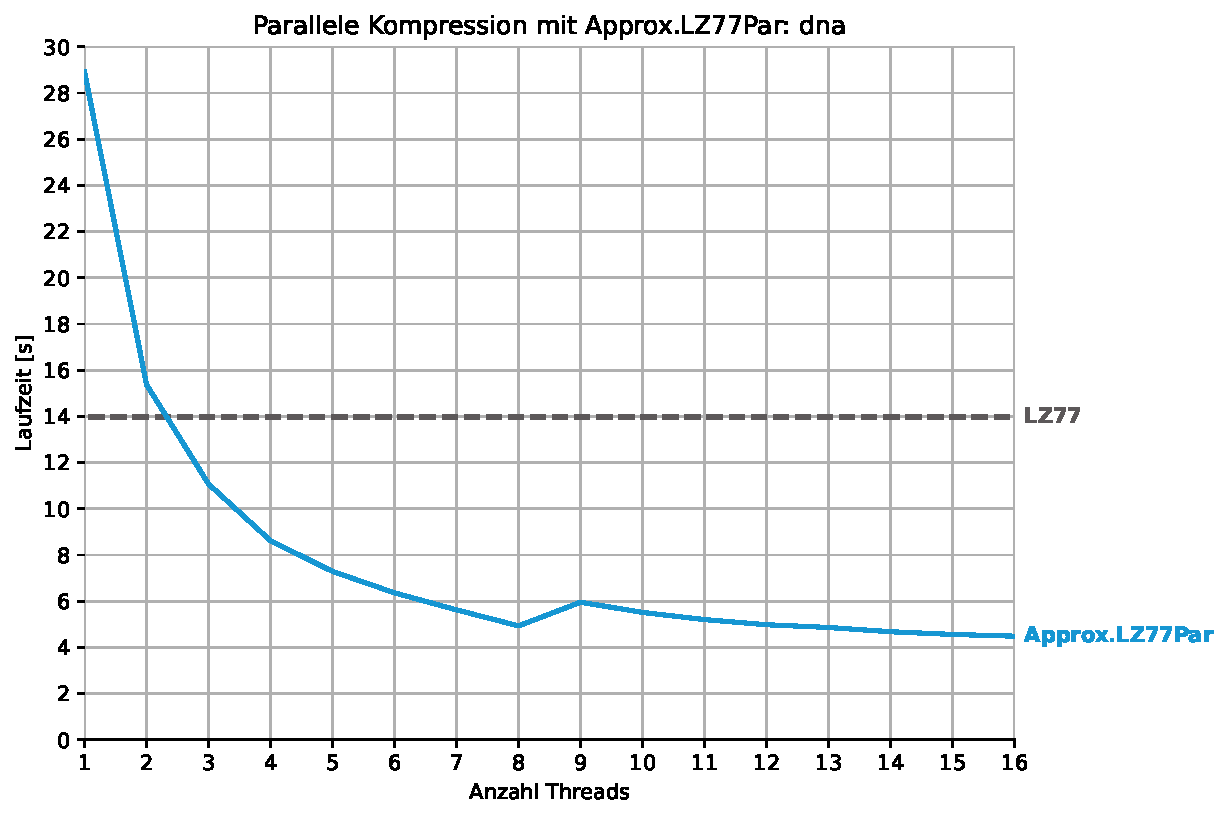
\includegraphics[scale=0.65]{Images/progressive_speedup_dna.pdf}
\end{figure}

\begin{figure}[H]
    \centering
    \caption{Laufzeitmessung von LZ77, Approx.LZ77 und Approx.LZ77Par(16 Threads) auf verschiedenen Präfixen von xml. Als Vergleichsmaß wurde 
    die lineare Regression der Kurven gestrichelt eingezeichnet.}
    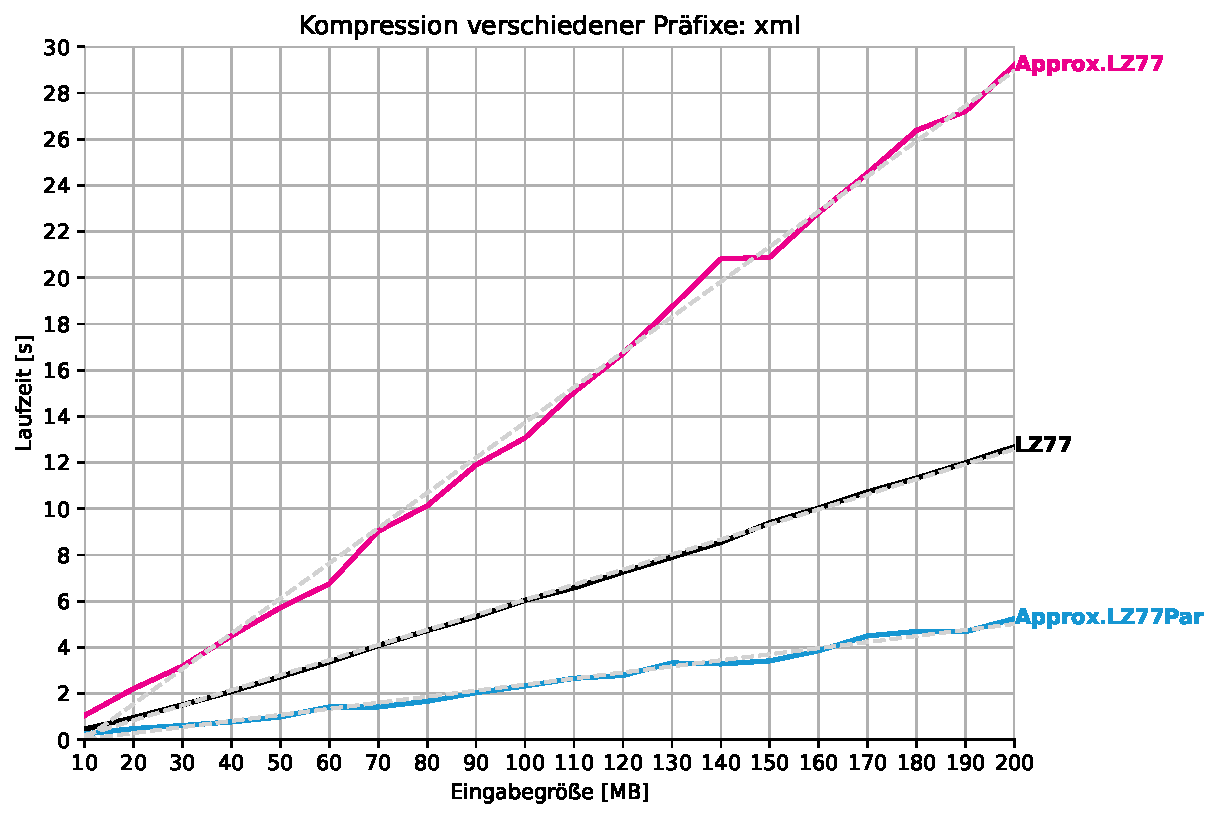
\includegraphics[scale=0.65]{Images/progressive_xml.pdf}
\end{figure}

\begin{figure}[H]
    \centering
    \caption{Laufzeitmessung von Approx.LZ77Par mit verschiedener Anzahl an Threads für xml}
    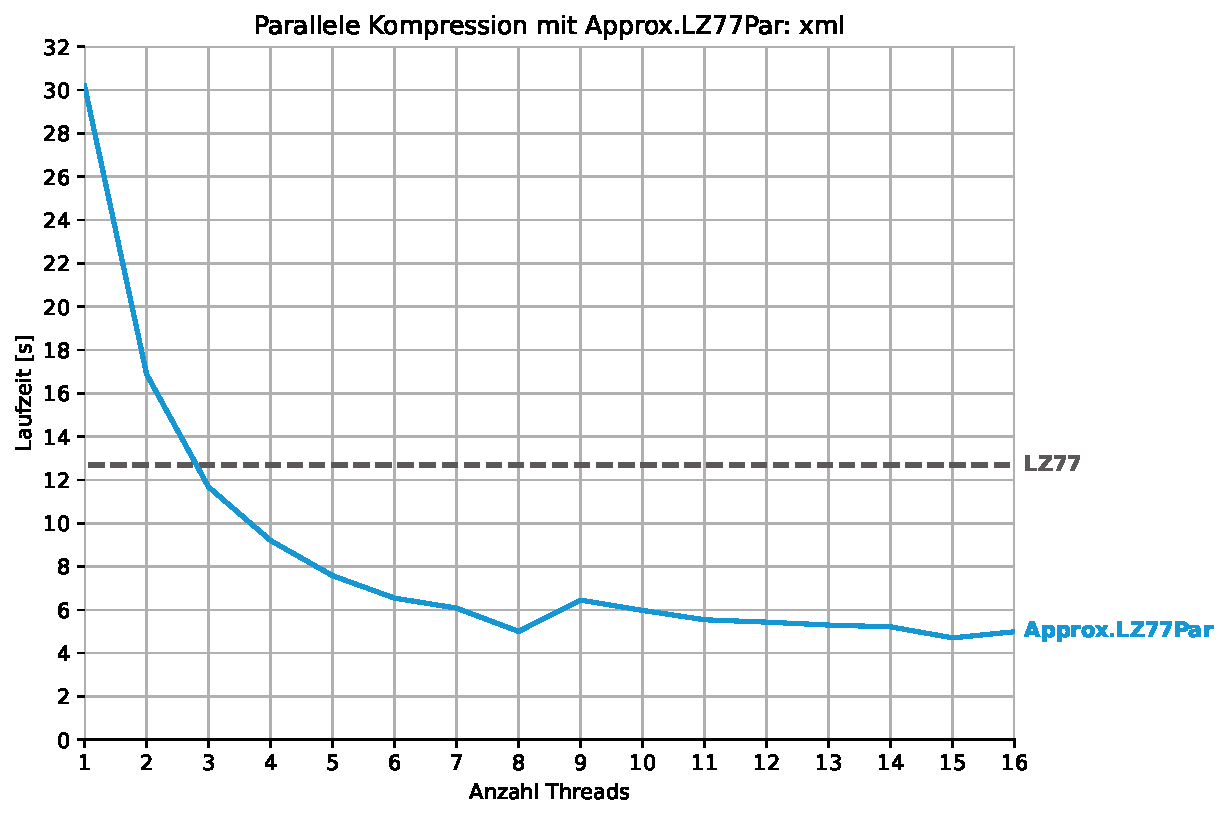
\includegraphics[scale=0.65]{Images/progressive_speedup_xml.pdf}
\end{figure}
\pagebreak
\section{Alternative Testumgebung}
Für die folgenden Messwerte wurden die Algorithmen auf einem Rechner mit einem AMD EYPC 7452 32-Core Prozessor mit 128 nutzbaren Threads ausgeführt.
Die Einstellungen der Algorithmen, die in \ref{settings} etabliert wurden, wurden beibehalten.

\begin{table}[ht]
    \centering
    \caption{Messwerte der Algorithmen auf verschiedenen Eingabedateien}
    \begin{tabular} { |c|c|c|c|c|c| }
        \hline
        \textbf{Eingabe} & \textbf{Algorithmus} & \textbf{Laufzeit[s]} & \textbf{Speicher} & \textbf{FR} & \textbf{CR*} \\
        \hline
        & LZ77 & 30.65 & 14.88 & 9.95\% & 70.92\% \\
        proteins & Approx.LZ77 & 64.46 & 9.94 & 15.34\% & 63.95\% \\
        & Approx.LZ77Par & 4.75 & 9.20 & 15.34\% & 63.95\% \\
        \hline
        & LZ77 & 28.38 & 13.44 & 5.50\% & 39.20\% \\
        sources & Approx.LZ77 & 62.35 & 6.42 & 10.05\% & 40.14\% \\
        & Approx.LZ77Par & 3.86 & 5.51 & 10.05\% & 40.14\% \\
        \hline
        & LZ77 & 33.59 & 13.44 & 6.66\% & 47.45\% \\
        english & Approx.LZ77 & 81.21 & 7.06 & 10.42\% & 43.39\% \\
        & Approx.LZ77Par & 4.30 & 5.95 & 10.42\% & 43.39\% \\
        \hline
        & LZ77 & 28.66 & 13.44 & 6.66\% & 47.46\% \\
        dna & Approx.LZ77 & 46.06 & 8.38 & 10.71\% & 45.53\% \\
        & Approx.LZ77Par & 3.52 & 6.13 & 10.71\% & 45.53\% \\
        \hline
        & LZ77 & 27.89 & 12.72 & 3.35\% & 23.89\% \\
        xml & Approx.LZ77 & 49.88 & 3.46 & 6.62\% & 26.78\% \\
        & Approx.LZ77Par & 2.91 & 3.28 & 6.62\% & 26.78\% \\
        \hline
    \end{tabular}
\end{table}

%%%%%%%%%%%%%%%%%%%%%%%%%%%%
%% Eidesstattliche Erklärung
%% muss angepasst werden 
%% in Erklaerung.tex
%%%%%%%%%%%%%%%%%%%%%%%%%%%%
\newpage
\thispagestyle{empty}
\section*{Eidesstattliche Erklärung}
\thispagestyle{empty}
Ich versichere hiermit an Eides statt, dass ich die vorliegende Abschlussarbeit mit dem oben genannten Titel selbstständig und ohne unzulässige fremde Hilfe erbracht habe. Ich habe keine anderen als die angegebenen Quellen und Hilfsmittel benutzt sowie wörtliche und sinngemäße Zitate kenntlich gemacht. Die Arbeit hat in gleicher oder ähnlicher Form noch keiner Prüfungsbehörde vorgelegen.
\vspace{4\baselineskip}\\
Dortmund, \today \hfill Autorname mit Unterschrift
\vspace{4\baselineskip}\\

\end{document}
